% !TEX root = main.tex
\subsubsection{Contextual bandits not in the exponential family: Oracle TS}
\label{sssec:evaluation_mixture_scenarios_oracle}

We further scrutinize Algorithm~\ref{alg:nonparametric_ts} by comparing it to \texttt{Oracle TS} algorithms for \texttt{Scenarios A}, \texttt{B}, \texttt{C} and \texttt{D}.
We implement separate \texttt{Oracle TS} algorithms for each scenario, via a Dirichlet prior distribution that has knowledge of the true underlying dimensionality $K_a$ per-arm.

This approach is similar to~\cite{ip-Urteaga2018}, where mixtures of Gaussian distributions model per-arm reward functions.
To provide a fair comparison to our proposed method, and instead of the variational inference-based original approach of~\citet{ip-Urteaga2018}, we implement a Gibbs sampler as described in Section~\ref{sec:proposed_method} where for each \texttt{Oracle TS}, the correct $K_a$ per-scenario is known (instead of the Dirichlet process prior assumed by \texttt{Nonparametric TS}).

We compare the performance of our proposed nonparametric Thompson sampling to that of each per-scenario \texttt{Oracle TS} in Figure~\ref{fig:mixture_scenarios_oracle}.
The proposed nonparametric Thompson sampling provides satisfactory performance across all studied scenarios, when compared to an unrealistic \texttt{Oracle TS} that knows the true number of underlying mixtures of the problem it is targeted to.

% Nonparametric and Oracle in scenarios
\begin{figure*}[!h]
	\centering
	\begin{subfigure}[c]{0.45\textwidth}
		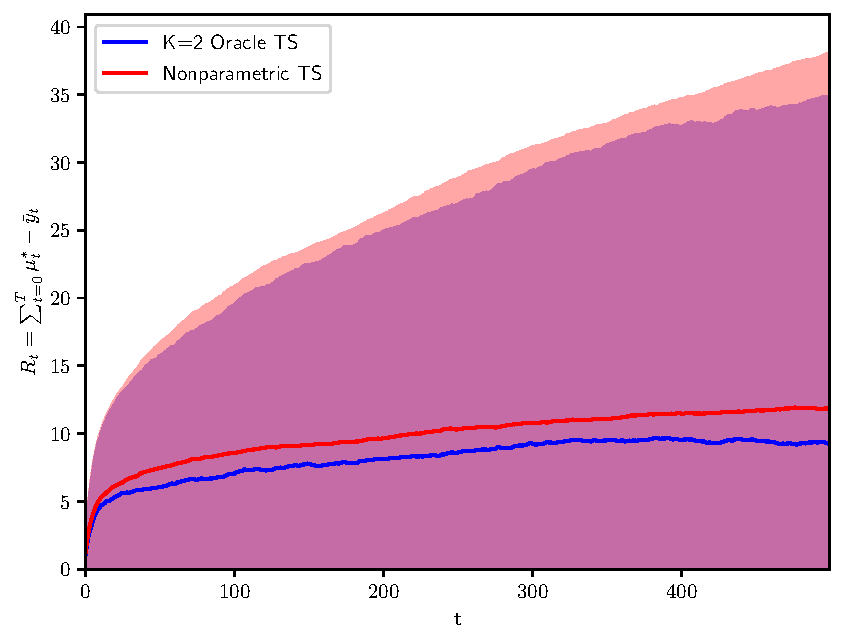
\includegraphics[width=\textwidth]{./figs/linearGaussianMixture/easy/cumregret_R3742.pdf}
		\vspace*{-5ex}
		\caption{\texttt{Scenario A}.}
		\label{fig:scenario_A_oracle}
	\end{subfigure}
	\begin{subfigure}[c]{0.45\textwidth}
		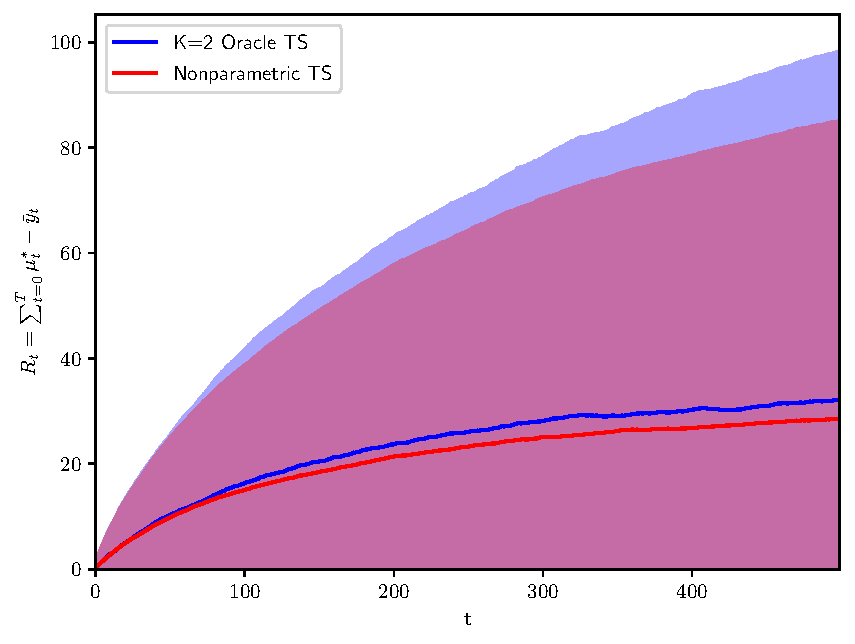
\includegraphics[width=\textwidth]{./figs/linearGaussianMixture/hard/cumregret_R3629.pdf}
		\vspace*{-5ex}
		\caption{\texttt{Scenario B}.}
		\label{fig:scenario_B_oracle}
	\end{subfigure}
	
	\begin{subfigure}[c]{0.45\textwidth}
		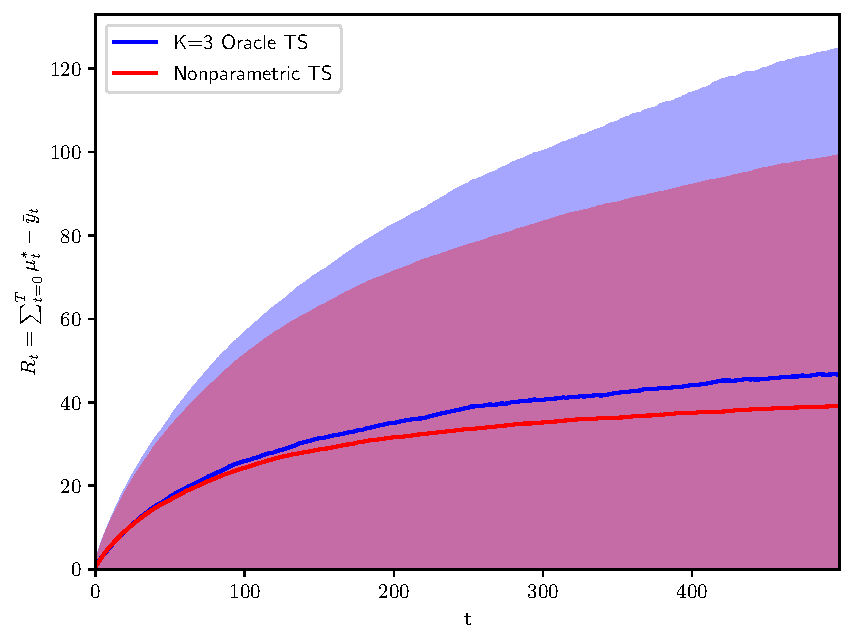
\includegraphics[width=\textwidth]{./figs/linearGaussianMixture/unbalanced/cumregret_R3641.pdf}
		\vspace*{-5ex}
		\caption{\texttt{Scenario C}.}
		\label{fig:scenario_C_oracle}
	\end{subfigure}
	\begin{subfigure}[c]{0.45\textwidth}
		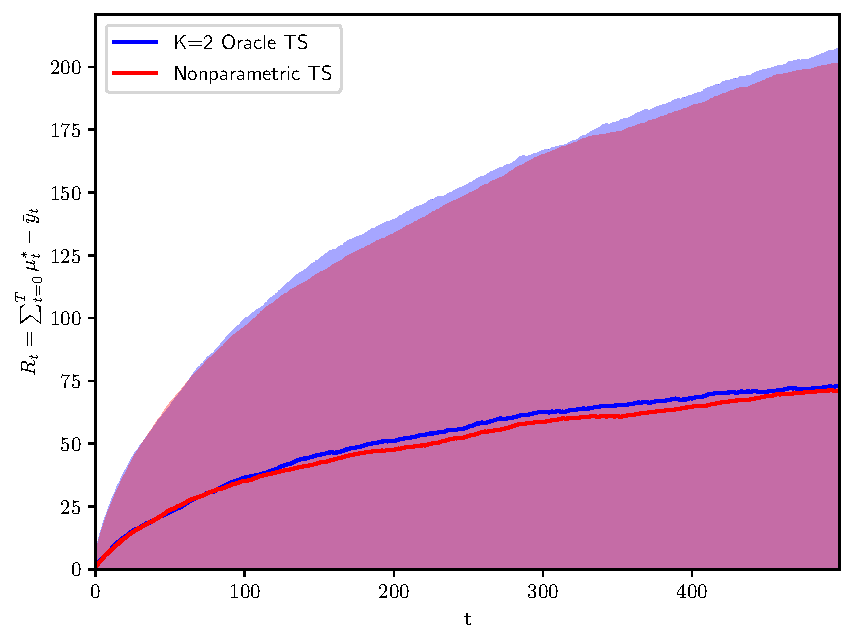
\includegraphics[width=\textwidth]{./figs/linearGaussianMixture/heavy/cumregret_R3250}
		\vspace*{-5ex}
		\caption{\texttt{Scenario D}.}
		\label{fig:scenario_D_oracle}
	\end{subfigure}
	\vspace*{-2ex}
	\caption{Mean regret (standard deviation shown as shaded region) for $R=3000$ realizations of the proposed and \texttt{Oracle TS} methods.}
	\label{fig:mixture_scenarios_oracle}
	\vspace*{-2ex}
\end{figure*}

The \texttt{Nonparametric TS} fits the underlying reward function accurately in all cases, attaining comparable regret in all scenarios.
We emphasize that the \texttt{Nonparametric TS} method does not demand any per-scenario hyperparameter tuning, and avoids model misspecification: \ie the same algorithm is used for all scenarios, while scenario specific \texttt{Oracle TS} methods are required.

These results demonstrate the competitive advantage of Bayesian nonparametrics to adjust the complexity of the reward model to the sequentially observed bandit data.
The proposed nonparametric generative modeling provides per-arm reward understanding (by plotting or computing figures of merit from these distributions), as the learned per-arm posteriors converge to the true posteriors.
We note that nonparametric posterior density convergence does not imply that it is consistent in $K$ ---on data from a finite mixture, nonparametric posteriors do not necessarily concentrate at the true number of components~\citep{j-Miller2014}. Nevertheless, we argue that density convergence suffices in the bandit setting.

% Misspecification, moved here for a better placement in the article
\begin{figure}[!h]
	\centering
	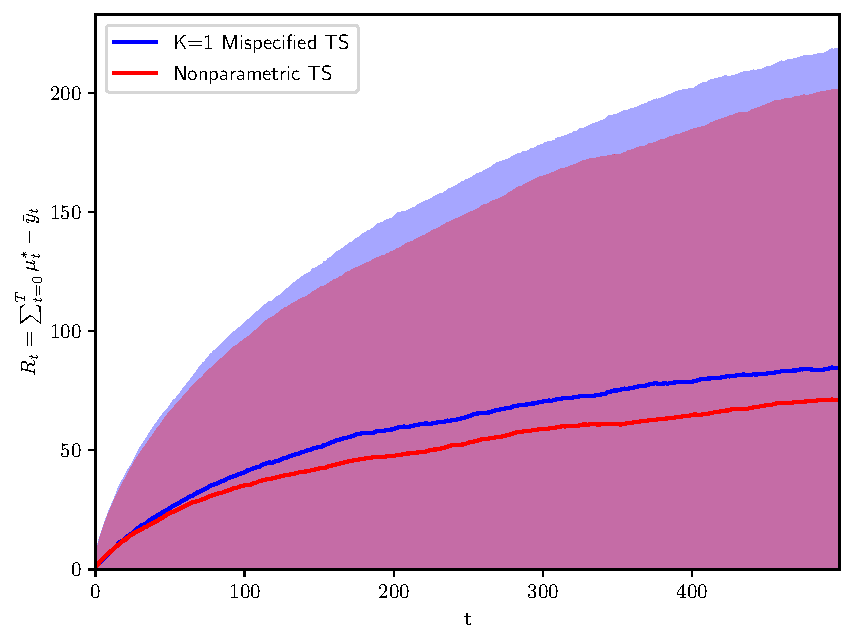
\includegraphics[width=0.75\textwidth]{./figs/linearGaussianMixture/heavy/cumregret_R3250_mispecified}
	\vspace*{-5ex}
	\caption{Mean regret (standard deviation shown as shaded region) for $R=3000$ realizations of the proposed and \texttt{Oracle TS} methods in \texttt{Scenario D} under model misspecification.}
	\label{fig:mixture_scenarios_misspecified}
	\vspace*{-2ex}
\end{figure}

We further highlight the built-in flexibility of the proposed nonparametric method by showing in Figure~\ref{fig:mixture_scenarios_misspecified} how Thompson sampling with a mispecified model (\ie fitting a unimodal Gaussian distribution to the heavy-tailed \texttt{Scenario D}) suffers in comparison to the proposed nonparametric method: a \%18 cumulative regret reduction is attained by \texttt{Nonparametric TS}.
With this, we reiterate the robustness and generality of our proposed nonparametric method in avoiding model-misspecification, a significant advantage for real-life bandit settings.